\documentclass{beamer}

\usepackage{tikz}
\usepackage{ngerman}
\usepackage{listings}
\usepackage{graphicx}

\usepackage{py_vortrag}


% title
\title{Einf"uhrung in Python}

\date{Juni 2010}

\author{Rebecca Breu}

\institute
{
 Verteilte Systeme und Grid-Computing \\
 JSC\\
 Forschungszentrum J"ulich
}


\begin{document}

\AtBeginPart
{
  \begin{frame}
  \titlepage
  \end{frame}

  \begin{frame}{Inhalt --- \insertpart}
  \tableofcontents
  \end{frame}
}


\AtBeginSection[]
{
   \begin{frame}{\insertsection}
       \tableofcontents[currentsection]
   \end{frame}
}


\begin{frame}
\titlepage
\end{frame}

\begin{frame}{Inhalt}
\begin{columns}[t]

\begin{column}{0.4\textwidth}
  Teil 1:\\[3mm]
  \tableofcontents[part=1]
\end{column}

\begin{column}{0.6\textwidth}
  Teil 2:\\[3mm]
  \tableofcontents[part=2]
  \vspace{7mm}
  Teil 3:\\[3mm]
  \tableofcontents[part=3]
\end{column}

\end{columns}
\end{frame}


\part{Teil 1}

\section{Introduction}

\begin{frame}{What is Python?}
\alert{Python:} dynamic programming language which supports several different programing paradigms:
\begin{itemize}
\item procedural programming
\item object oriented programming
\item functional programming
\end{itemize}
Standard: Python byte code is executed in the Python interpreter (similar to Java)\\
$\rightarrow$ \alert{platform independent code}
\end{frame}

\begin{frame}{Why Python?}
\begin{itemize}
\item syntax is clear, easy to read and learn (almost pseudo code)
\item intuitive object oriented programming
\item full modularity, hierarchical packages
\item error handling via exceptions
\item dynamic, high level data types
\item comprehensive standard library for many tasks
\item simply extendable via C/C++, wrapping of C/C++ libraries
\end{itemize}
\alert{Focus: programming speed}
\end{frame}

\begin{frame}{Is Python fast enough?}
\begin{itemize}
\item for compute intensive algorithms: Fortran, C, C++ might be better
\item for user programs: Python is fast enough!
\item most parts of Python are written in C
\item performance-critical parts can be re-implemented in C/C++ if necessary
\item first analyse, then optimise!
\end{itemize}
\end{frame}

\begin{frame}[fragile]{Hello World!}
\begin{lstlisting}[style=Python]
#!/usr/bin/env python

# This is a commentary
print "Hello world!"
\end{lstlisting}
\begin{lstlisting}[style=Shell]
$ python hello_world.py
Hello world!
$
\end{lstlisting}%$
\begin{lstlisting}[style=Shell]
$ chmod 755 hello_world.py
$ ./hello_world.py
Hello world!
$
\end{lstlisting} %$
\end{frame}

\begin{frame}[fragile]{Hello User}
\begin{lstlisting}[style=Python]
#!/usr/bin/env python

name = raw_input("What's your name? ")
print "Hello", name
\end{lstlisting}
\begin{lstlisting}[style=Shell]
$ ./hello_user.py
What's your name? Rebecca
Hello Rebecca
$
\end{lstlisting}
\end{frame}

\begin{frame}{Strong and Dynamic Typing}
\alert{Strong Typing:}
\begin{itemize}
\item Object is of exactly one type! A string is always a string, an integer always an integer
\item Counter examples: PHP, JavaScript, C: \texttt{char} can be interpreted as \texttt{short}, \texttt{void~*} can be everything
\end{itemize}
\alert{Dynamic Typing:}
\begin{itemize}
\item no variable declaration
\item variable names can be assigned to different data types in the course of a program
\item An object's attributes are checked only at run time
\end{itemize}
\end{frame}

\begin{frame}[fragile]{Strong and Dynamic Typing}
\begin{lstlisting}[style=Python]
number = 3
print number, type(number)
print number + 42
number = "3"
print number, type(number)
print number + 42
\end{lstlisting}
\begin{lstlisting}[style=Shell]
3 <type 'int'>
45
3 <type 'str'>
Traceback (most recent call last):
  File "test.py", line 6, in ?
    print number + 42
TypeError: cannot concatenate 'str' and 
'int' objects
\end{lstlisting}
\end{frame}

\begin{frame}[fragile]{Interactive Mode}
The interpreter can be started in interactive mode:
\begin{lstlisting}[style=Shell]
$ python
Python 2.6 (r26:66714, Feb  3 2009, 20:52:03) 
[GCC 4.3.2] on linux2
Type "help", "copyright", "credits" or ...
>>> print "hello world"
hello world
>>> a = 3 + 4
>>> print a
7
>>> 3 + 4
7
>>>
\end{lstlisting} %$
\end{frame}

\begin{frame}{Documentation}
Online help in the interpreter:
\begin{itemize}
\item \alert{\lstinline{help()}}: general Python help
\item \alert{\lstinline{help(obj)}}: help regarding an object, e.g. a function or a module
\item \alert{\lstinline{dir()}}: all used names
\item \alert{\lstinline{dir(obj)}}: all attributes of an object
\end{itemize}
\vspace{5mm}
Official documentation: \href{http://docs.python.org/}{http://docs.python.org/}
\end{frame}

\begin{frame}[fragile]{Documentation}
\begin{lstlisting}[style=Shell]
>>> help(dir)
Help on built-in function dir:
...
>>> a = 3
>>> dir()
['__builtins__', '__doc__', '__file__', 
'__name__', 'a']
>>> help(a)
Help on int object:
...
\end{lstlisting}
\end{frame}


\section{Datentypen I}

\begin{frame}[fragile]
\frametitle{Numerische Datentypen}
\begin{itemize}
\item \texttt{int}: entspricht \texttt{long} in C
\item \texttt{long}: unbegrenzter Wertebereich
\item \texttt{float}: enspricht \texttt{double} in C 
\item \texttt{complex}: komplexe Zahlen
\end{itemize} 
\begin{lstlisting}[style=Python]
a = 1
b = 1L
c = 1.0; c = 1e0
d = 1 + 0j
\end{lstlisting}
\vspace{3mm}
Integers werden bei Bedarf automatisch in long umgewandelt! 
\end{frame}

\begin{frame}
\frametitle{Operatoren auf Zahlen}
\begin{itemize}
\item Grundrechenarten: \texttt{+}, \texttt{-}, \texttt{*}, \texttt{/}
\item Div- und Modulo-Operator: \texttt{//}, \hspace{1mm}\texttt{\%}, \hspace{1mm}\texttt{divmod(x, y)}
\item Betrag: \texttt{abs(x)}
\item Runden: \texttt{round(x)}
\item Konvertierung: \texttt{int(x)}, \texttt{long(x)}, \texttt{float(x)}, \texttt{complex(re~[, im=0])}
\item Konjugierte einer komplexen Zahl: \texttt{x.conjugate()}
\item Potenzen: \texttt{x ** y}, \hspace{1mm}\texttt{pow(x, y)}
\end{itemize}
Ergebnis einer Verkn"upfung unterschiedlicher Datentypen ist vom Typ des \glqq gr"o"seren\grqq \, Datentyps.
\end{frame}

\begin{frame}[fragile]
\frametitle{Strings}
Datentyp: \texttt{str}
\begin{itemize}
\item \lstinline{s = 'spam'}, \lstinline{s = "spam"}
\item Mehrzeilige Strings: \lstinline{s = """spam"""}
\item keine Interpretation von Escape-Sequenzen: \lstinline{s = r"spam"}
\item Strings aus anderen Datentypen erzeugen: \lstinline{str(1.0)}
\end{itemize}
\begin{lstlisting}[style=Shell]
>>> print "sp\nam"
sp
am
>>> print r"sp\nam"
sp\nam
>>> s = """hallo
... welt"""
>>> print s
hallo
welt
\end{lstlisting}
\end{frame}

\begin{frame}
\frametitle{String-Methoden}
\begin{itemize}
\item Vorkommen von Substrings z"ahlen: \lstinline{s.count(sub [, start[, end]])}
\item beginnt/endet s mit einem Substring? \lstinline{s.startswith(sub[, start[, end]])}, \lstinline{s.endswith(sub[, start[, end]])}
\item s in Gro"s-/Kleinbuchstaben: \lstinline{s.upper()}, \lstinline{s.lower()}
\item Leerraum entfernen: \lstinline{s.strip([chars])}
\item an Substrings trennen: \lstinline{s.split([sub [,maxsplit]])}
\item Position eines Substrings finden: \lstinline{s.index(sub[, start[, end]])}
\item einen Substring ersetzen: \lstinline{s.replace(old, new[, count])}
\end{itemize}
Weitere Methoden: \lstinline{help(str)}, \lstinline{dir(str)}
\end{frame}

\begin{frame}
\frametitle{Listen}
Datentyp: \texttt{list}
\begin{itemize}
\item \lstinline{s = [1, "spam", 9.0, 42]}, \lstinline{s = []}
\item Element anh"angen: \lstinline{s.append(x)}
\item um zweite Liste erweitern: \lstinline{s.extend(s2)}
\item Vorkommen eines Elements z"ahlen: \lstinline{s.count(x)}
\item Position eines Elements: \lstinline{s.index(x[, min[, max]])}
\item Element an Position einf"ugen: \lstinline{s.insert(i, x)}
\item Element an Position l"oschen und zur"uckgeben: \lstinline{\s.pop([i])}
\item Element l"oschen: \lstinline{s.remove(x)}
\item Liste umkehren: \lstinline{s.reverse()}
\item Sortieren: \lstinline{s.sort([cmp[, key[, reverse]]])}
\item Summe der Elemente: \lstinline{sum(s)}
\end{itemize}
\end{frame}

\begin{frame}
\frametitle{Operationen auf Sequenzen}
Stings und Listen haben viel gemeinsam: Sie sind \alert{Sequenzen}.
\begin{itemize}
\item Ist ein Element in s enhalten/nicht enthalen?\\
 \lstinline{x in s}, \lstinline{x not in s}
\item Sequenzen aneinanderh"angen: \lstinline{s + t}
\item Sequenzen vervielf"altigen: \lstinline{n * s}, \lstinline{s * n}
\item i-tes Element: \lstinline{s[i]}, von hinten: \lstinline{s[-i]}
\item Subsequenz: \lstinline{s[i:j]}, mit Schrittweite k: \lstinline{s[i:j:k]}
\item Subsequenz von Anfgang/bis Ende: \lstinline{s[:-2]}, \lstinline{s[2:]}, \lstinline{s[:]}
\item L"ange: \lstinline{len(s)}
\item kleinstes/gr"o"stes Element: \lstinline{min(s)}, \lstinline{max(s)}
\item Zuweisungen: \lstinline{(a, b, c) = s} \\
$\rightarrow$ \lstinline{a = s[0]}, \lstinline{b = s[1]}, \lstinline{c = s[2]}
\end{itemize}
\end{frame}

\begin{frame}[fragile]
\frametitle{Sequenzen}
\begin{itemize}
\item Auch eine Sequenz: Datentyp \alert{\texttt{tuple}}: a = (1, 2, 3)
\item Listen sind ver"anderbar
\item Strings und Tupel sind nicht ver"anderbar
\begin{itemize}
\item Keine Zuweisung \lstinline{s[i] = ...}
\item Kein Anh"angen und L"oschen von Elementen
\item Funktionen wie \texttt{upper} liefern einen neuen String zur"uck!
\end{itemize}
\end{itemize}
\begin{lstlisting}[style=Shell]
>>> s1 = "spam"
>>> s2 = s1.upper()
>>> s1
'spam'
>>> s2
'SPAM'
\end{lstlisting}
\end{frame}

\begin{frame}[fragile]
\frametitle{Referenzen}
\begin{itemize}
\item In Python ist alles eine Referenz auf ein Objekt!
\item Vorsicht bei Zuweisungen:
\end{itemize}
\begin{lstlisting}[style=Shell]
>>> s1 = [1, 2, 3, 4]
>>> s2 = s1
>>> s2[1] = 17
>>> s1
[1, 17, 3, 4]
>>> s2
[1, 17, 3, 4]
\end{lstlisting}
Flache Kopie einer Liste: \lstinline{s2 = s1[:]} oder \lstinline{s2 = list(s1)}
\end{frame}

\begin{frame}[fragile]
\frametitle{Wahrheitswerte}
Datentyp \alert{bool}: \texttt{True}, \texttt{False}

Werte, die zu \texttt{False} ausgewertet werden:
\begin{itemize}
\item \texttt{None}
\item \texttt{False}
\item \texttt{0} (in jedem numerischen Datentyp)
\item leere Strings, Listen und Tupel: \texttt{''}, \texttt{()}, \texttt{[]}
\item leere Dictionaries: \texttt{\{\}}
\item leere Sets
\end{itemize}
Andere Objekte von eingebauten Datentypen werden stets zu \texttt{True} ausgewertet!
\begin{lstlisting}[style=Shell]
>>> bool([1, 2, 3])
True
>>> bool("")
False
\end{lstlisting}
\end{frame}

%%% Local Variables: 
%%% mode: latex
%%% latex-run-command: pdflatex
%%% TeX-master: "vortrag"
%%% End: 

\section{Statements}

\begin{frame}[fragile]{Das if-Statement}
\begin{lstlisting}[style=Python]
if a == 3:
    print "Aha!"
\end{lstlisting}
\begin{itemize}
\item Bl"ocke werden durch Einr"uckung festgelegt!
\item Standard: Einr"uckung mit vier Leerzeichen
\end{itemize}
\begin{lstlisting}
if a == 3:
    print "spam"
elif a == 10:
    print "eggs"
elif a == -3:
    print "bacon"
else:
    print "something else"
\end{lstlisting}
\end{frame}

\begin{frame}[fragile]{Vergleichsoperatoren}
\begin{itemize}
\item Vergleich des Inhalts: \texttt{==}, \texttt{<}, \texttt{>}, \texttt{<=}, \texttt{>=}, \texttt{!=}
\item Vergleich der Objektidentit"at: \lstinline{a is b}, \lstinline{a is not b}\item Und/Oder-Verkn"upfung: \lstinline{a and b}, \lstinline{a or b}
\item Negation: \lstinline{not a}
\end{itemize}
\begin{lstlisting}
if not (a==b) and (c<3):
    pass
\end{lstlisting}
\end{frame}

\begin{frame}[fragile]{Conditional Expressions}
Kurze Schreibweise f"ur bedingte Zuweisung. Statt:
\begin{lstlisting}
if zahl<0:
    s = "Negativ"
else:
    s = "Positiv"
\end{lstlisting}
kann man schreiben:
\begin{lstlisting}
s = "Negativ" if zahl<0 else "Positiv"
\end{lstlisting}
\end{frame}

\begin{frame}[fragile]{for-Schleifen}
\begin{lstlisting}[style=Python]
for i in range(10):
    print i   # 0, 1, 2, 3, ..., 9

for i in range(3, 10):
   print i    # 3, 4, 5, ..., 9

for i in range(0, 10, 2):
   print i   # 0, 2, 4, ..., 8
else:
   print "Schleife komplett durchlaufen."
\end{lstlisting}
\begin{itemize}
\item Schleife vorzeitig beenden: \lstinline{break}
\item n"achster Durchlauf: \lstinline{continue}
\item \lstinline{else} wird ausgef"uhrt, wenn die Schleife nicht vorzeitig verlassen wurde
\end{itemize}
\end{frame}

\begin{frame}[fragile]
"Uber Sequenzen kann man direkt (ohne Index) iterieren:
\begin{lstlisting}[style=Python]
for item in ["spam", "eggs", "bacon"]:
    print item
\end{lstlisting}

Auch die \texttt{range}-Funktion liefert eine Liste:
\begin{lstlisting}[style=Shell]
>>> range(0, 10, 2)
[0, 2, 4, 6, 8]
\end{lstlisting}
Ben"otigt man doch Indices:
\begin{lstlisting}[style=Python]
for (i, char) in enumerate("hallo welt"):
    print i, char
\end{lstlisting}
\end{frame}

\begin{frame}[fragile]{while-Schleifen}
\begin{lstlisting}[style=Python]
while i < 10:
    i += 1
\end{lstlisting}
Auch hier k"onnen \lstinline{break} und \lstinline{continue} verwendet werden.\\[3mm]
Ersatz f"ur do-while-Schleife:
\begin{lstlisting}[style=Python]
while True:
   # wichtiger Code
   if bedingung:
       break
\end{lstlisting} 
\end{frame}


\section{Funktionen}

\begin{frame}[fragile]{Funktionen}
\begin{lstlisting}[style=Python]
def addiere(a, b):
    """Gibt die Summe von a und b zurueck."""

    summe = a + b
    return summe
\end{lstlisting}

\begin{lstlisting}[style=Shell]
>>> ergebnis = addiere(3, 5)
>>> print ergebnis
8
>>> help(addiere)
Help on function addiere in module __main__:

addiere(a, b)
    Gibt die Summe von a und b zurueck.
\end{lstlisting}
\end{frame}

\begin{frame}[fragile]{R"uckgabewerte und Parameter}
\begin{itemize}
\item Funktionen k"onnen beliebige Objekte als Parameter und R"uckgabewerte haben
\item Typen der R"uckgabewerte und Parameter sind nicht festgelegt
\item Funktionen ohne expliziten R"uckgabewert geben \lstinline{None} zur"uck
\end{itemize}
\begin{lstlisting}[style=Python]
def hallo_welt():
    print "Hallo Welt!"

a = hallo_welt()
print a
\end{lstlisting}
\begin{lstlisting}[style=Shell]
$ mein_programm.py
Hallo Welt
None
\end{lstlisting} %$
\end{frame}

\begin{frame}[fragile]{Mehrere R"uckgabewerte}
Mehrere R"uckgabewerte werden mittels Tupel oder Listen realisiert:
\begin{lstlisting}[style=Python]
def foo():
   a = 17
   b = 42
   return (a, b)

ret = foo()
(x, y) = foo()
\end{lstlisting}
\end{frame}

\begin{frame}[fragile]{Keywords und Defaultwerte}
Man kann Parameter auch in anderer Reihenfolge als definiert angeben:
\begin{lstlisting}[style=Python]
def foo(a, b, c):
    print a, b, c

foo(b=3, c=1, a="hallo")
\end{lstlisting}
Defaultwerte festlegen:
\begin{lstlisting}[style=Python]
def foo(a, b, c=1.3):
    print a, b, c

foo(1, 2)
foo(1, 17, 42)
\end{lstlisting}
\end{frame}

\begin{frame}[fragile]{Funktionen sind Objekte}
Funktionen sind Objekte und k"onnen wie solche zugewiesen und "ubergeben werden:
\begin{lstlisting}[style=Shell]
>>> a = float
>>> a(22)
22.0
\end{lstlisting}
\begin{lstlisting}[style=Shell]
>>> def foo(fkt):
...     print fkt(33)
...
>>> foo(float)
33.0
\end{lstlisting}
\end{frame}


\newpage

\section*{Input/Output}
\begin{aufgabe}[String formatting]
Start the Python interpreter.
\begin{auflistung}
\item Display \lstinline{float} numbers with a given number of positions before and after decimal point, and in exponential notation.
\item Display \lstinline{int} numbers in hexadecimal and octal notation.
\item Given a person's given name, family name, residence and age, display the data in one line, e.g.:
\begin{verbatim}
"James Kirk is 35 years old and lives in Iowa."
\end{verbatim}
\item Try more formatting possibilities: \texttt{\underline{http://docs.python.org/lib/typesseq-strings.html}}
\end{auflistung}
\end{aufgabe}

\begin{aufgabe}[Command line parameters]
Write a program which prints its name and all its command line parameters.
\end{aufgabe}

\begin{aufgabe}[Read files]
Write a program which counts the frequency of the word "spam" in a file. \hinweis{There's a useful string method!}
\end{aufgabe}

\begin{aufgabe}[Read and write files]
Write a program which reads a file, adds a line number to each of its lines and writes the ouput to a new file. Example output:
\begin{verbatim}
1. Hallo
2. Welt
\end{verbatim}

\end{aufgabe}



%%\section*{Module}

%%\begin{aufgabe}
%%\end{aufgabe}


%%% Local Variables: 
%%% mode: latex
%%% TeX-master: "uebung1"
%%% End: 

\section{Errors and Exceptions}

\begin{frame}[fragile]{Syntax Errors, Indentation Errors}
Errors while parsing: \alert{Program doesn't get executed}. E.g.: 
\begin{itemize}
\item Mismatched or missing parenthesis
\item Missing or misplaced semicolons, colons, commas
\item Indentation errors
\end{itemize}
\begin{lstlisting}[style=Python]
print "I'm running..."
def add(a, b)
   return a + b
\end{lstlisting}
\begin{lstlisting}[style=Shell]
$ ./add.py
  File "add.py", line 2
    def add(a, b)
                ^
SyntaxError: invalid syntax
\end{lstlisting} %$
\end{frame}

\begin{frame}[fragile]{Exceptions}
Exceptions occur at \alert{runtime}:
\begin{lstlisting}[style=Python]
import math
print "I'm running..."
math.foo()
\end{lstlisting}
\begin{lstlisting}[style=Shell]
$ ./test.py
I'm running...
Traceback (most recent call last):
  File "test.py", line 3, in ?
    math.foo()
AttributeError: 'module' object has no 
attribute 'foo'
\end{lstlisting} %$
\end{frame}

\begin{frame}[fragile]{Handling Exceptions}
\begin{lstlisting}[style=Python]
try:
    s = raw_input("Enter a number: ")
    number = float(s)
except ValueError:
    print "That's not a number!"
\end{lstlisting}
\begin{itemize}
\item \lstinline{except} block is executed when the code in the code in the \lstinline{try}-Block throws an according exception
\item afterwards, the program continues normally
\item unhandled exceptions force the program to exit.
\end{itemize}
Handling different kinds of exceptions:
\begin{lstlisting}[style=Python]
except (ValueError, TypeError, NameError):
\end{lstlisting}
\end{frame}

\begin{frame}[fragile]{Handling Exceptions}
\begin{lstlisting}[style=Python]
try:
    s = raw_input("Enter a number: ")
    number = 1/float(s)
except ValueError:
    print "That's not a number!"
except ZeroDivisionError:
    print "You can't divide by zero!"
except:
    print "Oops, what's happened?"
\end{lstlisting}
\begin{itemize}
\item Several \lstinline{except} statements for different exceptions
\item Last \lstinline{except} can be used without specifying the kind of exception: Catches all remaining exceptions
\begin{itemize}
\item Careful: Can mask unintended programming errors!
\end{itemize}
\end{itemize}
\end{frame}

\begin{frame}[fragile]{Handling Exceptions}
\begin{itemize}
\item \alert{\texttt{else}} is executed if no exception occurred
\item \alert{\texttt{finally}} is executed \alert{in any} case
\end{itemize}
\begin{lstlisting}[style=Python]
try:
    f = open("spam")
except IOError:
    print "Cannot open file"
else:
    print f.read()
    f.close()
finally:
    print "End of try."
\end{lstlisting}
\end{frame}

\begin{frame}[fragile]{Exception Objects}
Access to exception objects:
\begin{lstlisting}[style=Python]
try:
    f = open("spam")
except IOError, e:
    print e.errno, e.strerror
    print e
\end{lstlisting}
\begin{lstlisting}[style=Shell]
$ python test.py
2 No such file or directory
[Errno 2] No such file or directory: 'spam'
\end{lstlisting}%$
\end{frame}

\begin{frame}{Exceptions in Function Calls}
\begin{figure}
\centering
\only<1>
{
  \begin{tikzpicture}
  \draw [black] (0, 0.2) node {draw()};
  \draw [white, ->] (0, 0) arc(180:270:15pt) node[anchor=west] {rectangle()};
  \draw [white, ->] (1.5, -0.7) arc(180:270:15pt) 
                    -- (2.5, -1.23) node[anchor=west] {line()};
  \draw [white] (4.6, -1.23) node {Exception!};
  \draw [white, ->] (4.5, -1.0) arc(0:90:15pt) -- (2.8, -0.47);
  \draw [white, ->] (2.6, -0.3) arc(0:90:15pt) -- (0.8, 0.225);
  \end{tikzpicture}
}

\only<2>
{
  \begin{tikzpicture}
  \draw [black] (0, 0.2) node {draw()};
  \draw [black, ->] (0, 0) arc(180:270:15pt) node[anchor=west] {rectangle()};
  \draw [white, ->] (1.5, -0.7) arc(180:270:15pt) 
                    -- (2.5, -1.23) node[anchor=west] {line()};
  \draw [white] (4.6, -1.23) node {Exception!};
  \draw [white, ->] (4.5, -1.0) arc(0:90:15pt) -- (2.8, -0.47);
  \draw [white, ->] (2.6, -0.3) arc(0:90:15pt) -- (0.8, 0.225);
  \end{tikzpicture}
}

\only<3>
{
  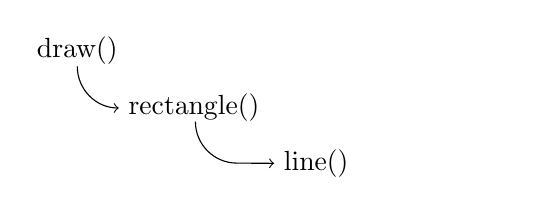
\begin{tikzpicture}
  \draw [black] (0, 0.2) node {draw()};
  \draw [black, ->] (0, 0) arc(180:270:15pt) node[anchor=west] {rectangle()};
  \draw [black, ->] (1.5, -0.7) arc(180:270:15pt) 
                    -- (2.5, -1.23) node[anchor=west] {line()};
  \draw [white] (4.6, -1.23) node {Exception!};
  \draw [white, ->] (4.5, -1.0) arc(0:90:15pt) -- (2.8, -0.47);
  \draw [white, ->] (2.6, -0.3) arc(0:90:15pt) -- (0.8, 0.225);
  \end{tikzpicture}
}

\only<4>
{
  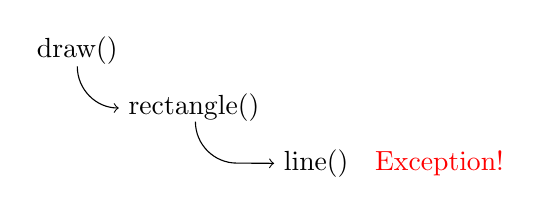
\begin{tikzpicture}
  \draw [black] (0, 0.2) node {draw()};
  \draw [black, ->] (0, 0) arc(180:270:15pt) node[anchor=west] {rectangle()};
  \draw [black, ->] (1.5, -0.7) arc(180:270:15pt) 
                    -- (2.5, -1.23) node[anchor=west] {line()};
  \draw [red] (4.6, -1.23) node {Exception!};
  \draw [white, ->] (4.5, -1.0) arc(0:90:15pt) -- (2.8, -0.47);
  \draw [white, ->] (2.6, -0.3) arc(0:90:15pt) -- (0.8, 0.225);
  \end{tikzpicture}
}

\only<5>
{
  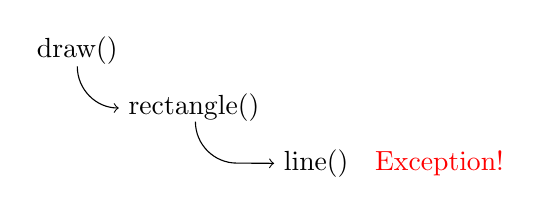
\begin{tikzpicture}
  \draw [black] (0, 0.2) node {draw()};
  \draw [black, ->] (0, 0) arc(180:270:15pt) node[anchor=west] {rectangle()};
  \draw [black, ->] (1.5, -0.7) arc(180:270:15pt) 
                    -- (2.5, -1.23) node[anchor=west] {line()};
  \draw [red] (4.6, -1.23) node {Exception!};
  \draw [white, ->] (4.5, -1.0) arc(0:90:15pt) -- (2.8, -0.47);
  \draw [white, ->] (2.6, -0.3) arc(0:90:15pt) -- (0.8, 0.225);
  \end{tikzpicture}
}

\only<6>
{
  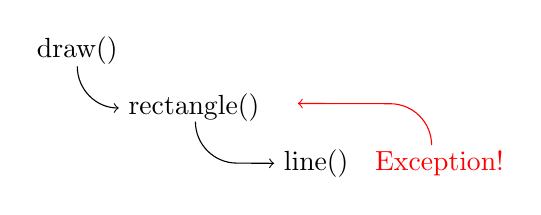
\begin{tikzpicture}
  \draw [black] (0, 0.2) node {draw()};
  \draw [black, ->] (0, 0) arc(180:270:15pt) node[anchor=west] {rectangle()};
  \draw [black, ->] (1.5, -0.7) arc(180:270:15pt) 
                    -- (2.5, -1.23) node[anchor=west] {line()};
  \draw [red] (4.6, -1.23) node {Exception!};
  \draw [red, ->] (4.5, -1.0) arc(0:90:15pt) -- (2.8, -0.47);
  \draw [white, ->] (2.6, -0.3) arc(0:90:15pt) -- (0.8, 0.225);
  \end{tikzpicture}
}

\only<7>
{
  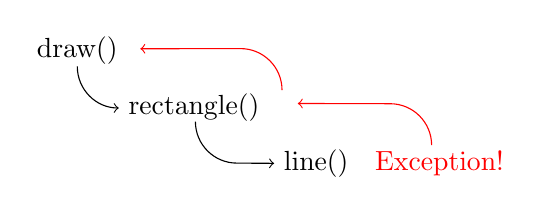
\begin{tikzpicture}
  \draw [black] (0, 0.2) node {draw()};
  \draw [black, ->] (0, 0) arc(180:270:15pt) node[anchor=west] {rectangle()};
  \draw [black, ->] (1.5, -0.7) arc(180:270:15pt) 
                    -- (2.5, -1.23) node[anchor=west] {line()};
  \draw [red] (4.6, -1.23) node {Exception!};
  \draw [red, ->] (4.5, -1.0) arc(0:90:15pt) -- (2.8, -0.47);
  \draw [red, ->] (2.6, -0.3) arc(0:90:15pt) -- (0.8, 0.225);
  \end{tikzpicture}
}
\end{figure}
\begin{itemize}
\item<1-> Function calls another function.
\item<4-> That function raises an exception.
\item<5-> Is exception handled?
\item<6-> No: Pass exception to calling function.
\end{itemize}
\end{frame}

\begin{frame}[fragile]{Raising Exceptions}
Passing exceptions on:
\begin{lstlisting}[style=Python]
try:
    f = open("spam")
except IOError:
    print "Problem while opening file!"
    raise
\end{lstlisting}
\vspace{3mm}
Raising exceptions:
\begin{lstlisting}[style=Python]
def gauss_solver(matrix):
    # Important code
    raise ValueError("Singular matrix")
\end{lstlisting}
\end{frame}


\begin{frame}[fragile]{Exceptions vs. Checking Values Beforehand}
\onslide<1->
Exceptions are preferable!

\begin{lstlisting}
def square(x):
    if type(x) == int or type(x) == float:
        return x ** 2
    else:
        return None
\end{lstlisting}
Bad!

\onslide<2->
\begin{itemize}
  \item What about other numerical data types (complex numbers, own data types)? Better: Try to compute the power and catch possible exceptions! $\rightarrow$ \alert{Duck-Typing}

  \item Caller of a function might forget to check return values for validity. Better: Raise an exception!
\end{itemize}
\end{frame}


\begin{frame}[fragile]{The \texttt{with} Statement}
Some objects offer context management, which provides a more convenient way to write \lstinline{try ... finally} blocks:
\begin{lstlisting}
with open("test.txt") as f:
    for line in f:
        print line
\end{lstlisting}
After the \lstinline{with} block the file object is guaranteed to be closed properly, no matter what exceptions occurred within the block.\vspace{5mm}

In Python 2.5 this needs the following import:
\begin{lstlisting}
from __future__ import with_statement
\end{lstlisting}
\end{frame}


\vielspass

\part{Teil 2}
\section{Data Types II}

\begin{frame}[fragile]{Sets}
\alert{Set}: unordered, no duplicated elements
\begin{itemize}
\item \lstinline{s = set([sequence])}
\item \alert{Subset}: \lstinline{s.issubset(t)}, \lstinline{s <= t}, proper s.: \lstinline{s < t}
\item \alert{Superset}: \lstinline{s.issuperset(t)}, \lstinline{s >= t}, proper s.: \lstinline{s > t} 
\item \alert{Union}: \lstinline{s.union(t)}, \lstinline{s | t}
\item \alert{Intersection}: \lstinline{s.intersection(t)}, \lstinline{s & t}
\item \alert{Difference}: \lstinline{s.difference(t)}, \lstinline{s - t}
\item Symmetric Difference: \lstinline{s.symmetric_difference(t)}, \lstinline{s ^ t}
\item Copy: \lstinline{s.copy()}
\end{itemize}
As with sequences, the following works: \lstinline{x in set}, \lstinline{len(set)}, \lstinline{for x in set}, \lstinline{add}, \lstinline{remove}
\end{frame}

\begin{frame}[fragile]{Dictionaries}
\alert{Dictionary}: Mapping of key $\rightarrow$ value
\begin{lstlisting}[style=Shell]
>>> d = { "spam": 1, "eggs": 17}
>>> d["eggs"]
17
>>> d["bacon"] = 42
>>> d
{'eggs': 17, 'bacon': 42, 'spam': 1}
\end{lstlisting}
Iterating over dictionaries:
\begin{lstlisting}[style=Python]
for key in d:
    print key, d[key]
\end{lstlisting}
\end{frame}

\begin{frame}[fragile]{Operations on Dictionaries}
\begin{itemize}
\item Delete an entry: \lstinline{del}
\item Delete all entries: \lstinline{d.clear()}
\item Copy: \lstinline{d.copy()}
\item Does it contain a key? \lstinline{d.has_key(k)}, \lstinline{k in d}
\item List of all (key, value) tuples: \lstinline{d.items()}
\item List of all keys: \lstinline{d.keys()}
\item List all values: \lstinline{d.values()}
\item Get an entry: \lstinline{d.get(k[, x])}
\item Remove and return entry: \lstinline{d.pop(k[, x])}
\item Remove and return arbitrary entry:  \lstinline{d.popitem()}
\end{itemize}
\end{frame}




\section{Object Oriented Programming}

\begin{frame}{Object Oriented Programming}
\begin{itemize}
\item So far: \alert{procedural programming}
\begin{itemize}
\item Data
\item Functions taking data as parameters and returning results
\end{itemize}
\item Alternative: Group data and functions belonging together to form \alert{custom data types}
\item $\rightarrow$ Extensions of structures in C/Fortran
\end{itemize}
\end{frame}

\begin{frame}[fragile]{Using Simple Classes as Structs}
\begin{lstlisting}[style=Python]
class Point:
    pass

p = Point()
p.x = 2.0
p.y = 3.3
\end{lstlisting}
\begin{itemize}
\item \alert{Class}: Custom date type (here: \texttt{Point})
\item \alert{Object}: Instance of a class (here: \texttt{p})
\item Attributes (here \texttt{x}, \texttt{y}) can be added dynamically
\end{itemize}
\end{frame}

\begin{frame}[fragile]{Classes}
\begin{lstlisting}[style=Python]
class Point:
    def __init__(self, x, y):
        self.x = x
        self.y = y

p = Point(2.0, 3.0)
print p.x, p.y
p.x = 2.5
p.z = 42
\end{lstlisting}
\begin{itemize}
\item \texttt{\_\_init\_\_}: Is called automatically after creating an object
\end{itemize}
\end{frame}

\begin{frame}[fragile]{Methods on Objects}
\begin{lstlisting}[style=Python]
class Point:
    def __init__(self, x, y):
        self.x = x
        self.y = y

    def norm(self):
        n = math.sqrt(self.x**2 + self.y**2)
        return n

p = Point(2.0, 3.0)
print p.x, p.y, p.norm()
\end{lstlisting}
\begin{itemize}
\item Method call: automatically sets the object as first parameter
\item $\rightarrow$ traditionally called \lstinline{self}
\item\alert{Careful}: Overloading of methods not possible!
\end{itemize}
\end{frame}

\begin{frame}[fragile]{Converting Objects to Strings}
\onslide<1->
Default return value of \lstinline{str(...)} for objects of custom classes:
\begin{lstlisting}[style=Shell]
>>> p = Point(2.0, 3.0)
>>> print p  # --> print str(p)
<__main__.Point instance at 0x402d7a8c>
\end{lstlisting}
\vspace{2mm}

\onslide<2->
This behaviour can be overwritten:
\begin{lstlisting}[style=Python]
def __str__(self):
    return "(%i, %i)" % (self.x, self.y)
\end{lstlisting}
\begin{lstlisting}[style=Shell]
>>> print p
(2, 3)
 \end{lstlisting}
\end{frame}

\begin{frame}[fragile]{Comparing Objects}
\onslide<1->
Default: \texttt{==} checks for object identity of custom objects.
\begin{lstlisting}[style=Shell]
>>> p1 = Point(2.0, 3.0)
>>> p2 = Point(2.0, 3.0)
>>> p1 == p2
False
\end{lstlisting}
%\vspace{2mm}
\onslide<2->
This behaviour can be overwritten:
\begin{lstlisting}[style=Python]
def __eq__(self, other):
    return (self.x == other.x) and
           (self.y == other.y)
\end{lstlisting}
\begin{lstlisting}[style=Shell]
>>> p1 == p2 # Check for equal values
True
>>> p1 is p2 # Check for identity
False
\end{lstlisting}
\end{frame}

\begin{frame}[fragile]{Comparing Objects}
More relational operators:
\begin{itemize}
\item \texttt{<} : \lstinline{__lt__(self, other)}
\item \texttt{<=} : \lstinline{__le__(self, other)}
\item \texttt{!=} : \lstinline{__ne__(self, other)}
\item \texttt{>} : \lstinline{__gt__(self, other)}
\item \texttt{>=} : \lstinline{__ge__(self, other)}
\end{itemize}
\vspace{2mm}
Alternative: \lstinline{__cmp__(self, other)}, returns:
\begin{itemize}
\item negative integer when \lstinline{self < other}
\item zero when \lstinline{self == other}
\item positive integer when \lstinline{self > other}
\end{itemize}
\end{frame}

\begin{frame}{Emulating Existing Data Types}
Classes can emulate built-in data types:
\begin{itemize}
\item Numbers: arithmetics, \texttt{int(myobj)}, \texttt{float(myobj)}, \dots
\item Functions: \texttt{myobj(...)}
\item Sequences: \texttt{len(myobj)}, \texttt{myobj[...]}, \lstinline{x in myobj}, ...
\item Iterators: \lstinline{for i in myobj}
\end{itemize}
\vspace{2mm}
See documentation:\\
\href{http://docs.python.org/ref/specialnames.html}{http://docs.python.org/ref/specialnames.html}
\end{frame}

\begin{frame}[fragile]{Class Variables}
Have the same value for all instances of a class:
\begin{lstlisting}[style=Python]
class Point:
    count = 0  # Count all point objects
    def __init__(self, x, y):
        self.__class__.count += 1
        ...
\end{lstlisting}
\begin{lstlisting}[style=Shell]
>>> p1 = Point(2, 3); p2 = Point(3, 4)
>>> p1.count
2
>>> p2.count
2
>>> Point.count
2
\end{lstlisting}
\end{frame}

\begin{frame}[fragile]{Class Methods and Static Methods}
\begin{lstlisting}[style=Python]
class Spam:
    spam = "I don't like spam."

    @classmethod
    def cmethod(cls):
        print cls.spam
       
    @staticmethod
    def smethod():
        print "Blah blah."
\end{lstlisting}
\begin{lstlisting}[style=Python]
Spam.cmethod()
Spam.smethod()
s = Spam()
s.cmethod()
s.smethod()
\end{lstlisting}
\end{frame}

\begin{frame}{Inheritance}
There are often classes that are very similar to each other.\\
\alert{Inheritance} allows for:
\begin{itemize}
\item Hierarchical class structure (is-a-relationship)
\item Reusing of similar code
\end{itemize}
\vspace{5mm}
Example: Different types of phones
\begin{itemize}
\item Phone
\item Mobile phone (is a phone with additional functionality)
\item Smart phone (is a mobile phone with additional functionality)
\end{itemize}
\end{frame}

\begin{frame}[fragile]{Inheritance}
\begin{lstlisting}[style=Python]
class Phone:
    def call(self):
        pass

class MobilePhone(Phone):
    def send_text(self):
        pass
\end{lstlisting}
MobilePhone now inherits methods and attributes from Phone.
\begin{lstlisting}[style=Python]
h = MobilePhone()
h.call() # inherited from Phone
h.send_text() # own method
\end{lstlisting}
\end{frame}

\begin{frame}[fragile]{Overwriting Methods}
Methods of the parent class can be overwritten in the child class:
\begin{lstlisting}[style=Python]
class MobilePhone(Phone):
    def call(self):
        find_signal()
        Phone.call(self)
\end{lstlisting}
\end{frame}

\begin{frame}[fragile]{Multiple Inheritance}
Classes can inherit from multiple parent classes. Example:
\begin{itemize}
\item SmartPhone is a mobile phone
\item SmartPhone is a camera
\end{itemize}
\begin{lstlisting}[style=Python]
class SmartPhone(MobilePhone, Camera)
    pass

h = SmartPhone()
h.call()  # inherited from MobilePhone
h.take_photo() # inherited from Camera
\end{lstlisting}
Attributes are searched for in the following order:

SmartPhone, MobilePhone, parent class of MobilePhone (recursively), Camera, parent class of Camera (recursively).
\end{frame}

\begin{frame}[fragile]{Private Attributes}
\begin{itemize}
\item There are no private variables or private methods in Python.
\item \alert{Convention:} Mark attributes that shouldn't be accessed from outside with an underscore: \lstinline{_foo}.
\item To avoid name conflicts during inheritance: Names of the form \lstinline{__foo} are replaced with \lstinline{_classname__foo}:
\end{itemize}
\begin{lstlisting}[style=Python]
class Spam:
    __eggs = 3
\end{lstlisting}
\begin{lstlisting}[style=Shell]
>>> dir(Spam)
>>> ['_Spam__eggs', '__doc__', '__module__']
\end{lstlisting}
\end{frame}

\begin{frame}[fragile]{Properties}
If certain actions (checks, conversions) are to be executed while accessing attributes, use \alert{getter} and \alert{setter}:
\begin{lstlisting}[style=Python]
class Spam(object):
    def __init__(self):
        self._value = 0
    
    def get_value(self):
        return self._value

    def set_value(self, value):
        if value <= 0:  self._value = 0
        else:  self._value = value

    value = property(get_value, set_value)
\end{lstlisting}
\end{frame}

\begin{frame}[fragile]{Properties}
Properties can be accessed like any other attributes:
\begin{lstlisting}[style=Shell]
>>> s = Spam()
>>> s.value = 6   # set_value(6)
>>> s.value       # get_value()
>>> 6
>>> s.value = -6  # set_value(-6)
>>> s.value       # get_value()
>>> 0
\end{lstlisting}
\begin{itemize}
\item Getter and setter can be added later without changing the API
\item Access to \lstinline{_value} still possible
\end{itemize}

\end{frame}



\section{Python's Standard Library}

\begin{frame}{Python's Standard Library}
\alert{``Batteries included''}: comprehensive standard library for various tasks\\[4mm]

\includegraphics[height=4.5cm]{images/batteries_included.jpg}
\end{frame}

\begin{frame}[fragile]{Mathematics: \texttt{math}}
\begin{itemize}
\item Constants: \texttt{e}, \texttt{pi}
\item Round up/down: \texttt{floor(x)}, \texttt{ceil(x)}
\item Exponential function: \texttt{exp(x)}
\item Logarithm: \texttt{log(x[, base])}, \texttt{log10(x)}
\item Power and square root: \texttt{pow(x, y)}, \texttt{sqrt(x)}
\item Trigonometric functions: \texttt{sin(x)}, \texttt{cos(x)}, \texttt{tan(x)}
\item Conversion degree $\leftrightarrow$ radiant: \texttt{degrees(x)}, \texttt{radians(x)}
\end{itemize}
\begin{lstlisting}[style=Shell]
>>> import math
>>> math.sin(math.pi)
1.2246063538223773e-16
>>> math.cos(math.radians(30))
0.86602540378443871
\end{lstlisting}
\end{frame}


\begin{frame}[fragile]{Random Numbers: \texttt{random}}
\begin{itemize}
\item Random integers: \\ \texttt{randint(a, b)},  \texttt{randrange([start,] stop[, step])}
\item Random floats (uniform distr.): \texttt{random()}, \texttt{uniform(a, b)}
\item Other distibutions: \texttt{expovariate(lambd)}, \texttt{gammavariate(alpha, beta)}, \texttt{gauss(mu, sigma)}, \dots
\item Random element of a sequence: \texttt{choice(seq)}
\item Several unique, random elements of a sequence: \texttt{sample(population, k)}
\item Shuffled sequence: \texttt{shuffle(seq[, random])}
\end{itemize}
\begin{lstlisting}[style=Python]
>>> s = [1, 2, 3, 4, 5]
>>> random.shuffle(s)
>>> s
[2, 5, 4, 3, 1]
>>> random.choice("Hello world!")
'e'
\end{lstlisting}
\end{frame}


\begin{frame}[fragile]{Exact decimals: \texttt{fractions}}

\begin{lstlisting}
>>> from fractions import Fraction
>>> a = Fraction(2, 3)
>>> b = Fraction(2, 5)
>>> print float(a), float(b)
0.66666666666666663 0.40000000000000002
>>> a+b
Fraction(16, 15)
>>> a/b
Fraction(5, 3)
\end{lstlisting}

(See also: module \texttt{decimal}.)
\end{frame}


\begin{frame}[fragile]{Date and Time: \texttt{datetime}}
Date and time objects:
\begin{lstlisting}
d1 = datetime.date(2008, 3, 21)  
d2 = datetime.date(2008, 6, 22)
dt = datetime.datetime(2011, 8, 26, 12, 30)
t = datetime.time(12, 30)
\end{lstlisting}
Calculating with date and time:
\begin{lstlisting}
print d1 < d2
delta = d2 - d1
print delta.days
print d2 + datetime.timedelta(days=44)
\end{lstlisting}
\end{frame}

\begin{frame}[fragile]{More Data Types: \texttt{collections}}
\alert{defaulttict}: Dictionary which creates default values for non-existant keywords:
\begin{lstlisting}
frequency = defaultdict(lambda: 0)

for c in "Hello world!":
    frequency[c] += 1
\end{lstlisting}
Paramter (optional): function creating the default values
\end{frame}


\begin{frame}[fragile]{Operations on Path Names: \texttt{os.path}}
\begin{itemize}
\item Paths: \texttt{abspath(path)}, \texttt{basename(path)}, \texttt{normpath(path)}, \texttt{realpath(path)}
\item Construct paths: \texttt{join(path1[, path2[, ...]])}
\item Split paths: \texttt{split(path)}, \texttt{splitext(path)}
\item File information: \texttt{isfile(path)}, \texttt{isdir(path)}, \texttt{islink(path)}, \texttt{getsize(path)}, \dots
\item Expand home directory: \texttt{expanduser(path)}
\item Expand environment variables: \texttt{expandvars(path)}
\end{itemize} 
\begin{lstlisting}[style=Shell]
>>> os.path.join("spam", "eggs", "ham.txt")
'spam/eggs/ham.txt'
>>> os.path.splitext("spam/eggs.py")
('spam/eggs', '.py')
>>> os.path.expanduser("~/spam")
'/home/rbreu/spam'
>>> os.path.expandvars("/blah/$TEST")
'/bla/test.py'
\end{lstlisting}%$
\end{frame}

\begin{frame}[fragile]{Files and Directories: \texttt{os}}
\begin{itemize}
\item Working directory: \lstinline{getcwd()}, \lstinline{chdir(path)}
\item Changing file permissions: \lstinline{chmod(path, mode)}
\item Changing ower: \lstinline{chown(path, uid, gid)}
\item Creating directories: \lstinline{mkdir(path[, mode])}, \lstinline{makedirs(path[, mode])}
\item Removing files: \lstinline{remove(path)}, \lstinline{removedirs(path)}
\item Renaming files: \lstinline{rename(src, dst)}, \lstinline{renames(old, new)}
\item List of files in a directory: \lstinline{listdir(path)}
\end{itemize}
\begin{lstlisting}[style=Python]
for myfile in os.listdir("mydir"):
    os.chmod(os.path.join("mydir", myfile), 
             stat.S_IRUSR|stat.S_IWUSR)
\end{lstlisting}
\end{frame} 

\begin{frame}[fragile]{Directory Listing: \texttt{glob}}
List of files in a directory with Unix-like extension of wildcards: \texttt{glob(path)}
\begin{lstlisting}[style=Shell]
>>> glob.glob("python/[a-c]*.py")
['python/confitest.py',
 'python/basics.py',
 'python/curses_test2.py',
 'python/curses_keys.py',
 'python/cmp.py',
 'python/button_test.py',
 'python/argument.py',
 'python/curses_test.py']
\end{lstlisting}
\end{frame}

\begin{frame}[fragile]{Files and Directories: \texttt{shutil}}
Higher level operations on files and direcories.
\begin{itemize}
\item Copying files: \texttt{copyfile(src, dst)}, \texttt{copy(src, dst)}
\item Recursive copy: \texttt{copytree(src, dst[, symlinks])}
\item Recursive removal: \\\texttt{rmtree(path[, ignore\_errors[, onerror]])}
\item Recursive move: \texttt{move(src, dst)}
\end{itemize}
\begin{lstlisting}[style=Python]
shutil.copytree("spam/eggs", "../beans", 
                 symlinks=True)
\end{lstlisting}
\end{frame}

\begin{frame}[fragile]{Run Processes: \texttt{subprocess}}
Simple execution of a program:
\begin{lstlisting}[style=Python]
p = subprocess.Popen(["ls", "-l", "mydir"])
returncode = p.wait() # wait for p to end
\end{lstlisting}
Access to the program's output:
\begin{lstlisting}[style=Python]
p = Popen(["ls"], stdout=PIPE, stderr=STDOUT) 
p.wait()
output = p.stdout.read()
\end{lstlisting}
Pipes between processes (\lstinline{ls -l | grep txt})
\begin{lstlisting}[style=Python]
p1 = Popen(["ls", "-l"], stdout=PIPE)
p2 = Popen(["grep", "txt"], stdin=p1.stdout)
\end{lstlisting}
\end{frame}

\begin{frame}[fragile]{Access to Command Line Parameters: \texttt{optparse}}
\begin{itemize}
\item Simple list of parameters: $\rightarrow$ \texttt{sys.argv}
\item More convenient for handling several options: \texttt{OptionParser}
\end{itemize}
\begin{lstlisting}[style=Python]
parser = optparse.OptionParser()
parser.add_option("-f", "--file", 
                  dest="filename",
                  default="out.txt",
                  help="output file")
parser.add_option("-v", "--verbose",
                  action="store_true", 
                  dest="verbose", 
                  default=False,
                  help="verbose output")

(options, args) = parser.parse_args()
print options.filename, options.verbose
print args
\end{lstlisting}
\end{frame}
\begin{frame}[fragile]{Zugriff auf Kommandozeilenparameter: \texttt{optparse}}
Usage of an optparse program:
\begin{lstlisting}[style=Shell]
$ ./test.py -h
usage: test.py [options]

options:
  -h, --help     show this help message and exit
  -f FILENAME, --file=FILENAME
                 output file
  -v, --verbose  verbose output
\end{lstlisting} %$
\begin{lstlisting}[style=Shell]
$ ./test.py -f aa bb cc
aa False
['bb', 'cc']
\end{lstlisting} %$
\end{frame}

\begin{frame}[fragile]{Configuration Files: \texttt{ConfigParser}}
Simple format to store configuration etc: Windows' INI format
\begin{lstlisting}[style=Python]
[font]
font = Times New Roman
# comment (or: ! as comment symbol)
size = 16

[colors]
font = black
pointer = %(font)s
background = white
\end{lstlisting}
\end{frame}

\begin{frame}[fragile]{Configuration Files: \texttt{ConfigParser}}
Reading configuration files:
\begin{lstlisting}[style=Python]
parser = ConfigParser.SafeConfigParser()
parser.readfp(open("config.ini", "r"))
print parser.get("colors", "font")
\end{lstlisting}
More parser methods:
\begin{itemize}
\item List of all sections: \texttt{sections()}
\item List of all options: \texttt{options(section)}
\item List of all options and values: \texttt{items(section)}
\item Reading values: \texttt{get(sect, opt)}, \\
\texttt{getint(sect, opt)}, \texttt{getfloat(sect, opt)}, \texttt{getboolean(sect, opt)}
\end{itemize}
\end{frame}

\begin{frame}[fragile]{Config Files: \texttt{ConfigParser}}
Writing configuration files:
\begin{lstlisting}[style=Python]
parser = ConfigParser.SafeConfigParser()
parser.add_section("colors")
parser.set("colors", "font", "black")
parser.write(open("config.ini", "w"))
\end{lstlisting}
More parser methods:
\begin{itemize}
\item Adding a section: \texttt{add\_section(section)}
\item Deleting a section: \texttt{remove\_section(section)}
\item Adding an option: \texttt{set(section, option, value)}
\item Removing and option: \texttt{remove\_option(section, option)}
\end{itemize}
\end{frame}

\begin{frame}[fragile]{CSV Files: \texttt{csv}}
CSV: Comma Seperated Values
\begin{itemize}
\item Data tables in ASCII format
\item Columns are delimited by a predefined character (most often comma)
\end{itemize}
\begin{lstlisting}[style=Python]
reader = csv.reader(open("test.csv", "rb"))
for row in reader:
    for item in row: 
        print item
\end{lstlisting}
\begin{lstlisting}[style=Python]
writer = csv.writer(open(outfile, "wb"))
writer.writerow([1, 2, 3, 4])
\end{lstlisting}
\end{frame}

\begin{frame}[fragile]{CSV Files: \texttt{csv}}
Handling different kinds of formats (dialects):
\begin{lstlisting}[style=Python]
reader(csvfile, dialect='excel') # Default
writer(csvfile, dialect='excel_tab')
\end{lstlisting}
\vspace*{3mm}
Specifying individual format parameters:
\begin{lstlisting}[style=Python]
reader(csvfile, delimiter=";")
\end{lstlisting}
Further format parameters: \texttt{lineterminator}, \texttt{quotechar}, \texttt{skipinitialspace}, \dots
\end{frame}

\begin{frame}[fragile]{Serialising Objects: \texttt{pickle}}
Saving single, arbitrary objects in files:
\begin{lstlisting}[style=Python]
obj = {"hello": "world", "spam":1}
pickle.dump(obj, open("blah.bin", "wb"))
# ...
obj = pickle.load(open("blah.bin", "rb"))
\end{lstlisting}
Converting objects in strings (e.g. to send via streams):
\begin{lstlisting}[style=Python]
s = pickle.dumps(obj)
# ...
obj = pickle.loads(s)
\end{lstlisting}
\end{frame}

\begin{frame}[fragile]{Persistent Dictionaries: \texttt{shelve}}
A shelve is used like a dictionary; it saves its content to a file.
\begin{lstlisting}[style=Python]
d = shelve.open("blah")
d["spam"] = "eggs"
d["blah"] = 1
del d["foo"]   
d.close()  
\end{lstlisting}
\end{frame}

\begin{frame}[fragile]{Lightweight Database: \texttt{sqlite3}}
Database in a file or in memory; in Python's stdlib sine 2.5.
\begin{lstlisting}[style=Python]
conn = sqlite3.connect("bla.db")
c = conn.cursor()

c.execute("""CREATE TABLE Friends
             (firstname TEXT, lastname TEXT)""")
c.execute("""INSERT INTO Friends
             VALUES("Jane", "Doe")""")
conn.commit()
\end{lstlisting}
\begin{lstlisting}[style=Python]
c.execute("""SELECT * FROM Friends""")
for row in c: print row

c.close(); conn.close()
\end{lstlisting}
\end{frame}

\begin{frame}[fragile]{Lightweight Database: \texttt{sqlite3}}
String formatting is insecure since it allows injection of arbitrary SQL code!
\begin{lstlisting}[style=Python]
# Never do this!
symbol = "Jane"
c.execute("... WHERE firstname = '%s'" % symbol)
\end{lstlisting}
\vspace{2mm}
\includegraphics[width=\textwidth]{images/exploits_of_a_mom.png}
\end{frame}

\begin{frame}[fragile]{Lightweight Database: \texttt{sqlite3}}
Instead: Use the placeholder the database API provides:
\begin{lstlisting}[style=Python]
c.execute("... WHERE name = ?", symbol)
\end{lstlisting}
\begin{lstlisting}[style=Python]
f = (("Janis", "Joplin"), ("Bob", "Dylan"))
for item in friends:
    c.execute("""INSERT INTO Friends 
                 VALUES (?,?)""", item)
\end{lstlisting}
\end{frame}

\begin{frame}[fragile]{Tar Archives: \texttt{tarfile}}
Extracting a tgz:
\begin{lstlisting}[style=Python]
tar = tarfile.open("spam.tgz")
tar.extractall()
tar.close()
\end{lstlisting}
\vspace*{3mm}
Creating a tgz:
\begin{lstlisting}[style=Python]
tar = tarfile.open("spam.tgz", "w:gz")
tar.add("/home/rbreu/test")
tar.close()
\end{lstlisting}
\end{frame}

\begin{frame}[fragile]{Logging Output: \texttt{logging}}
Flexible output of information which can be easily customised.
\begin{lstlisting}[style=Python]
import logging
logging.debug("Very special information.")
logging.info("I am doing this and that.")
logging.warning("You should know this.")
\end{lstlisting}
\begin{lstlisting}[style=shell]
WARNING:root:You should know this.
\end{lstlisting}
\begin{itemize}
\item Messages are assigned a priority:\\
 \texttt{CRITICAL}, \texttt{ERROR}, \texttt{WARNING}, \texttt{INFO}, \texttt{DEBUG}
\item Default: Only messages with priority \texttt{WARNING} or higher are printed
\end{itemize}
\end{frame}

\begin{frame}[fragile]{Logging Output: \texttt{logging}}
Example: Output into file, custom format, higher logging level:
\begin{lstlisting}[style=Python, basicstyle=\ttfamily\small]
logging.basicConfig(level=logging.DEBUG,
  format="%(asctime)s %(levelname)-8s %(message)s",
  datefmt="%Y-%m-%d %H:%M:%S",
  filename='/tmp/spam.log', filemode='w')
\end{lstlisting}
\begin{lstlisting}[style=Shell, basicstyle=\ttfamily\small]
$ cat /tmp/spam.log
2007-05-07 16:25:14 DEBUG   Very special information.
2007-05-07 16:25:14 INFO    I am doing this and that.
2007-05-07 16:25:14 WARNING You should know this.
\end{lstlisting} %$
You can use multiple logger instancdes at the same time, see Python documentation.
\end{frame}

\begin{frame}[fragile]{Regul"are Ausdr"ucke: \texttt{re}}
Einfaches Suchen nach Mustern:
\begin{lstlisting}[style=Shell]
>>> re.findall(r"\[.*?\]", "a[bc]g[hal]def")
['[bc]', '[hal]']
\end{lstlisting}
\vspace*{2mm}
Ersetzen von Mustern:
\begin{lstlisting}[style=Shell]
>>> re.sub(r"\[.*?\]", "!", "a[bc]g[hal]def")
'a!g!def'
\end{lstlisting}
\vspace*{2mm}
Wird ein Regex-Muster mehrfach verwendet, sollte es aus Geschwindigkeitsgr"unden compiliert werden:
\begin{lstlisting}[style=Shell]
>>> pattern = re.compile(r"\[.*?\]")
>>> pattern.findall("a[bc]g[hal]def")
['[bc]', '[hal]']
\end{lstlisting}
\end{frame}

\begin{frame}[fragile]{Regul"are Ausdr"ucke: \texttt{re}}
Umgang mit Gruppen:
\begin{lstlisting}[style=Shell]
>>> re.findall("(\[.*?\])|(<.*?>)", 
               "[hi]s<b>sdd<hal>")
[('[hi]', ''), ('', '<b>'), ('', '<hal>')]
\end{lstlisting}
\vspace*{2mm}
Flags, die das Verhalten des Matching beeinflussen:
\begin{lstlisting}[style=Shell]
>>> re.findall("^a", "abc\nAbc", re.I|re.M)
>>> ['a', 'A']
\end{lstlisting}
\begin{itemize}
\item \texttt{re.I}: Gro"s-/Kleinschreibung ingnorieren
\item \texttt{re.M}: \lstinline{^} bzw. \lstinline{$} matchen am Anfang/Ende jeder Zeile (nicht nur am Anfang des Strings) %$
\item \texttt{re.S}: \lstinline{.} matcht auch Zeilenumbruch
\end{itemize}
\end{frame}


\begin{frame}[fragile]{URLs lesen: \texttt{urllib2}}
Einfaches lesen:
\begin{lstlisting}
import urllib2
r = urllib2.urlopen('http://www.fz-juelich.de')
print r.read()
print r.headers["content-type"]
\end{lstlisting}
Man kann den Request vorm Absenden anpassen:
\begin{lstlisting}
opener = urllib2.build_opener()
opener.addheaders = [('User-agent', 
                      'Mozilla/5.0')]
r = opener.open('http://www.fz-juelich.de')
\end{lstlisting}
Es werden Cookies, Authentifizierung, Proxies etc unterst"utzt.
\end{frame}


\begin{frame}[fragile]{XML-RPC-Client: \texttt{xmlrpclib}}
\begin{itemize}
\item XML-RPC: \alert{Remote Procedure Call} via XML und HTTP
\item unabh"anging von Plattform und Programmiersprache
\end{itemize}
\begin{lstlisting}[style=Python]
import xmlrpclib

s = xmlrpclib.Server("http://localhost:8000")
print s.add(2,3) 
print s.sub(5,2) 
\end{lstlisting}
Konvertierungen f"ur die g"angigen Datentypen geschehen automatisch: 
Booleans, Integer, Floats, Strings, Tupel, Listen, Dictionaries mit Strings als Keys, \dots
\end{frame}

\begin{frame}[fragile]{XML-RPC-Server: \texttt{SimpleXMLRPCServer}}
\begin{lstlisting}[style=Python]
from SimpleXMLRPCServer import SimpleXMLRPCServer

# Methoden, die der Server zur Verfuegung
# stellen soll:
class MyFuncs:
    def add(self, x, y):
        return x + y
    def sub(self, x, y):
        return x - y
    
# Erstelle und starte Server:
server = SimpleXMLRPCServer(("localhost", 8000))
server.register_instance(MyFuncs())
server.serve_forever()
\end{lstlisting}
\end{frame}





\vielspass

\part{Teil 3}
\section{Neues in Python 2.5}

\begin{frame}[fragile]
\frametitle{Conditional Expressions}
Kurze Schreibweise f"ur bedingte Zuweisung. Statt:
\begin{lstlisting}
if zahl<0:
    s = "Negativ"
else:
    s = "Positiv"
\end{lstlisting}
kann man schreiben:
\begin{lstlisting}
s = "Negativ" if zahl<0 else "Positiv"
\end{lstlisting}
\end{frame}

\begin{frame}[fragile]
\frametitle{Das \texttt{with}-Statement}
Einige Objekte bieten Kontext-Management an. Damit k"onnen \lstinline{try... finally}\,-Bl"ocke einfacher geschrieben werden:
\begin{lstlisting}
from __future__ import with_statement

with open("test.txt") as f:
    for line in f:
        print line
\end{lstlisting}
Nach dem \lstinline{with}-Block ist das Dateiobjekt stets wieder geschlossen, auch wenn im Block eine Exception auftrat.
\end{frame}

\begin{frame}[fragile]
\frametitle{Partielle Funktionsanwendung}
\begin{lstlisting}
import functools

def add (a, b):
    return a + b

add_ten = functools.partial(add, b=10)
add_ten(42)
\end{lstlisting}
\end{frame}

\section{Flexiblere Funktionen}

\begin{frame}[fragile]
\frametitle{Funktionsparameter aus Listen und Dictionaries}
\begin{lstlisting}
def spam(a, b, c, d):
    print a, b, c, d
\end{lstlisting}
Man kann positionale Parameter aus Listen erzeugen:
\begin{lstlisting}[style=Shell]
>>> args = [3, 6, 2, 3]
>>> spam(*args)
3 6 2 3
\end{lstlisting}
Man kann Keyword-Paramter aus Dictionaries erzeugen:
\begin{lstlisting}[style=Shell]
>>> kwargs = {"c": 5, "a": 2, "b": 4, "d":1}
>>> spam(**kwargs)
2 4 5 1
\end{lstlisting}
\end{frame}

\begin{frame}[fragile]
\frametitle{Funktionen mit beliebigen Parametern}
\begin{lstlisting}
def spam(*args, **kwargs):
    for i in args:
        print i
    for i in kwargs:
        print i, kwargs[i]
\end{lstlisting}
\begin{lstlisting}[style=Shell]
>>> spam(1, 2, c=3, d=4)
1
2
c 3
d 4
\end{lstlisting}
\end{frame}

\begin{frame}[fragile]
\frametitle{Anonyme Funktionen}
\begin{lstlisting}
def make_incrementor(n):
    return lambda x: x + n
\end{lstlisting}
\begin{lstlisting}[style=Shell]
>>> f = make_incrementor(42)
>>> f(0)
42
>>> f(1)
43
\end{lstlisting}
Sinnvoll, wenn einfache Funktionen als Parameter "ubergeben werden sollen.
\end{frame}

\section{Funktionale Techniken mit Listen}

\begin{frame}[fragile]
\frametitle{List Comprehension}
Abk"urzende Schreibweise zum Erstellen von Listen aus for-Schleifen. Statt:
\begin{lstlisting}
a = []
for i in range(10):
    a.append(i**2)
\end{lstlisting}
kann man schreiben:
\begin{lstlisting}
a = [i**2 for i in range(10)]
\end{lstlisting}
\end{frame}

\begin{frame}[fragile]
\frametitle{Map}
Anwenden einer Funktion auf alle Elemente einer Liste:
\begin{lstlisting}[style=Shell]
>>> a = [1.6, 4.0, 81.0, 9.0]
>>> map(math.sqrt, a)
[1.2649110640673518, 2.0, 9.0, 3.0]
>>> map(lambda x: x * 2, a)
[3.2000000000000002, 8.0, 162.0, 18.0]
\end{lstlisting}
Wenn die Funktion mehr als einen Parameter nimmt, kann je zus"atzlichem Parameter eine weitere Liste "ubergeben werden:
\begin{lstlisting}[style=Shell]
>>> map(math.pow, a, [2 for i in a])
[2.5600000000000005, 16.0, 6561.0, 81.0]
\end{lstlisting}
\end{frame} 

\begin{frame}[fragile]
\frametitle{Filter}
Gibt Elemente einer Liste zur"uck, die nach Anwendung einer Funktion wahr sind:
\begin{lstlisting}[style=Shell]
>>> a = [1, 2, 3, 4, 5, 6, 7, 8, 9]
>>> filter(lambda x: x % 2, a)
[1, 3, 5, 7, 9]
\end{lstlisting}
\end{frame}

\begin{frame}[fragile]
\frametitle{Reduce}
Wendet Funktion auf die ersten beiden Elemente an, dann auf das Ergebnis und das n"achste Element etc.
\begin{lstlisting}[style=Shell]
>>> def add(x, y):
...     return x + y
...
>>> a = [1, 2, 3, 4, 5, 6, 7, 8, 9]
>>> reduce(add, a)
45
\end{lstlisting}
Optionaler Startwert, der vor die Liste gesetzt wird:
\begin{lstlisting}[style=Shell]
>>> reduce(add, a, 10)
55
\end{lstlisting}
\end{frame}

\section{Iteratoren, Generatoren, Generator-Audr"ucke}

\begin{frame}[fragile]
\frametitle{Iteratoren}
Was passiert, wenn \lstinline{for} auf einem Objekt aufgerufen wird?
\begin{lstlisting}[style=Python]
for i in obj:
    pass
\end{lstlisting}
\begin{itemize}
\item Auf \lstinline{obj} wird die \lstinline{__iter__}-Methode aufgerufen, welche einen Iterator zur"uckgibt
\item Auf dem Iterator wird bei jedem Durchlauf \lstinline{next()} aufgerufen
\item Eine \lstinline{StopIteration}-Ausnahme beendet die for-Schleife
\end{itemize}
\end{frame}

\begin{frame}[fragile]
\frametitle{Iteratoren}
\begin{lstlisting}[style=Python]
class Reverse:
    def __init__(self, data):
        self.data = data
        self.index = len(data)
    def __iter__(self):
        return self
    def next(self):
        if self.index == 0:
            raise StopIteration
        self.index = self.index - 1
        return self.data[self.index]
\end{lstlisting}
\begin{lstlisting}[style=Shell]
>>> for char in Reverse("spam"):
...     print char,
...
m a p s
\end{lstlisting}
\end{frame}

\begin{frame}[fragile]
\frametitle{Generatoren}
Einfache Weise, Iteratoren zu erzeugen:
\begin{itemize}
\item Werden wie Funktionen definiert
\item \lstinline{yield}-Statement, um Daten zur"uckzugeben und beim n"achsten \lstinline{next}-Aufruf dort weiterzumachen
\end{itemize}
\begin{lstlisting}[style=Python]
def reverse(data):
    for index in range(len(data)-1, -1, -1):
        yield data[index]
\end{lstlisting}
\begin{lstlisting}[style=Shell]
>>> for char in reverse("spam"):
...     print char,
...
m a p s
\end{lstlisting}
\end{frame}

\begin{frame}[fragile]
\frametitle{Generator-Audr"ucke}
"Ahnlich zu List Comprehensions kann man anonyme Iteratoren erzeugen:
\begin{lstlisting}[style=Shell]
>>> data = "spam"
>>> for c in (data[i] for i in
...           range(len(data)-1, -1, -1)):
...     print c,
...
m a p s
\end{lstlisting}
\end{frame}


\section{Etwas Dynamik}
\begin{frame}[fragile]
\frametitle{Dynamische Attribute}
Erinnerung: Man kann Attribute von Objekten zur Laufzeit hinzuf"ugen:
\begin{lstlisting}
class Empty:
    pass

a = Empty()
a.spam = 42
a.eggs = 17
\end{lstlisting}
\vspace{2mm}
Und entfernen:
\begin{lstlisting}
del a.spam
\end{lstlisting}
\end{frame}

\begin{frame}[fragile]
\frametitle{getattr, setattr}
Man kann Attribute von Objekten als Strings ansprechen:
\begin{lstlisting}
import math
f = getattr(math, "sin")
print f(x) # sin(x)
\end{lstlisting}
\vspace{2mm}
\begin{lstlisting}
a = Empty()
setattr(a, "spam", 42)
print a.spam
\end{lstlisting}
N"utzlich, wenn man z.B. Attributnamen aus User-Input oder Dateien liest.
\end{frame}

%%% Local Variables: 
%%% mode: latex
%%% latex-run-command: pdflatex
%%% TeX-master: "vortrag"
%%% End: 

\section{Neues in Python 2.7}

\begin{frame}[fragile]{Neues in Python 2.7}

\begin{itemize}
\item Neue Syntax f"ur Mengen: Statt \texttt{set(1, 2, 3)} kann man schreiben: \texttt{\{1,2,3}\}
\item Analog zu List Comprehensions gibt es Set Comprehensions und Dictionary Comprehensions zum schnellen Erzeugen:
\begin{lstlisting}
s = {i*2 for in in range(3)}
d = {i: i*2 for i in range(3)}
\end{lstlisting}
\item \texttt{collections.OrderedDict}: Beim normalen Dictionary haben die Eintr"age eine willk"urliche Reihenfolge. OrderedDict kann die Eintr"age sortiert hinzuf"ugen.
\end{itemize}

\end{frame}

\section*{wxPython}

\begin{aufgabe}[Hello World]
\label{aufg-hello-world}Implement the Hello World application given in the lecture, creating an empty frame. Try different parameters for title, size and position of the frame.
\end{aufgabe}

\begin{aufgabe}[Static text]
\begin{teilaufgabe}
Extend the program from Exercise \ref{aufg-hello-world} so that it displays text inside the frame (\lstinline{wx.StaticText}). Display multi line text centered, as well as flushed left and flushed right.
\end{teilaufgabe}
\begin{teilaufgabe}
Add more \lstinline{wx.StaticText} widgets to the frame. What happens if you omit position parameters? Position the widgets via parameters and observe the behaviour of the frame on resizing.
\end{teilaufgabe}
\end{aufgabe}


\begin{aufgabe}[Buttons]
\begin{teilaufgabe}
Extend the program from Exercise \ref{aufg-hello-world} so that it displays a button. The program should exit when the button is pressed. (Close the main frame: \lstinline{self.Close(True)}.)
\end{teilaufgabe}
\begin{teilaufgabe}
Add more buttons. The buttons should execute different actions (e.g. print different text to the terminal) when clicked.
\end{teilaufgabe}
\end{aufgabe}

\begin{aufgabe}[Sizer]
\label{aufg-sizer}
Create a frame with a box sizer and buttons and try the different possibilities of box sizers. E.g.:
\begin{itemize}
\item A button that fills the whole frame
\item A horizontal row of buttons
\item A vertical row of buttons
\end{itemize}
You don't need to bind actions to the buttons; this exercise is all about layout.
\end{aufgabe}


\begin{aufgabe}[RadioBox]
\label{aufg-radiobox}
Create a frame which displays a radio box. As soon as the user selects one item, print the selection to the console.

\hinweis Contrary to the exercises above, it is now necessary to add the radio box object as an attribute to the frame object so that you can access it outside of the init method: \lstinline{self.radiobox = ...}
\end{aufgabe}

\begin{aufgabe}[Text editor]
Write a simple text editor. Proceed by the following steps:
\begin{teilaufgabe}[Text entry field]
Create a frame with a multiline TextCtrl widget. The text field should fill the whole frame, see Exercise \ref{aufg-sizer}. Try using the widget!
\begin{itemize}
\item What happens if you enter many lines into the field, or very long lines?
\item What do key combinations like Ctrl-C, Ctrl-V, Ctrl-X, Ins, Del, \dots do? 
\end{itemize}
\end{teilaufgabe}
\begin{teilaufgabe}[Menus]
Add a menu bar and a "File" menu. The menu should contain the entry "Quit".
\end{teilaufgabe}
\begin{teilaufgabe}[Status bar]
Add a status bar. Observe how the menu entry's help texts are automatically displayed in the status bar.
\end{teilaufgabe}
\begin{teilaufgabe}[New file]
Add a "New" entry to the status bar which deletes the content of the text entry field.

\hinweis Analogous to Exercise \ref{aufg-radiobox} you need to make the text entry field an attribute of the main frame object now.
\end{teilaufgabe}
\begin{teilaufgabe}[Open file]
Add an "Open \dots" entry to the file menu. The user should be able to select a file from a FileDialog which is then displayed in the text entry field.
\end{teilaufgabe}

\begin{teilaufgabe}[Save as]
Add a "Save as \dots" entry to the menu. The user should be able to select a file to wich the content of the text field entry is then saved.
\end{teilaufgabe}

\begin{teilaufgabe}[Save]
Add a "Save" entry to the menu bar, which saves the file under the name it was opend or saved last. In order to do that, add an attribute to the main frame  \lstinline{filename} which is updated accordingly on "Save as" and "Open".

Beware, the filename does not always exist when the user wants to save! (Why?) In this case, the \lstinline{filename} attribute should be \lstinline{None}; ideally the action "Save" invokes a file dialog in this case, as "Save as" does.

Additionally, you can display the filename in the frame's status bar (\lstinline{SetTitle}).
\end{teilaufgabe}

\begin{teilaufgabe}[Display in the status bar]
Display the program's actions in the status bar, e.g. "File blah.txt saved."
\end{teilaufgabe}

\begin{teilaufgabe}[Save status]
Save the status whether the file has been changed since being saved last in an attribute of the main frame. Display this status appropriately in the frame's title bar. The event triggered by the TextCtrl on text changes is \lstinline{wx.EVT_TEXT}.

Additionally you can add warnings (e.g. MessageDialog) when the user wants to execute "Open", "Quit" or "New" while having an unsaved file open.
\end{teilaufgabe}

\end{aufgabe}


\section{Zusammenfassung und Ausblick}

\begin{frame}{Zusammenfassung}
Wir haben kennengelernt:
\begin{itemize}
\item verschiedene \alert{Datentypen} (tw. \glqq High Level\grqq)
\item die wichtigsten \alert{Statements}
\item \alert{Funktion}sdeklaration und -Benutzung
\item \alert{Module} und Pakete
\item Fehler und \alert{Ausnahmen}, Behandlung selbiger
\item \alert{objektorientierte Programmierung}
\item einige h"aufig verwendete Standardmodule
\end{itemize}
\end{frame}

\begin{frame}{Offene Punkte}
Nicht behandelte, tw. fortgeschrittene Themen:
\begin{itemize}
\item Closures, Dekoratoren (Funktionswrapper)
\item Metaklassen
\item Weitere Standardmodule: Mail, WWW, XML, Zeit\&Datum, \dots $\rightarrow$~\href{http://docs.python.org/lib/modindex.html}{http://docs.python.org/lib/modindex.html}
\item Profiling, Debugging, Unittesting
\item Extending und Embedding: Python \& C/C++ $\rightarrow$~\href{http://docs.python.org/ext/ext.html}{http://docs.python.org/ext/ext.html}
\item Third Party-Module: Grafik, Webprogrammierung, Datenbanken, \dots $\rightarrow$~\href{http://pypi.python.org/pypi}{http://pypi.python.org/pypi}
\end{itemize}
\end{frame}

\begin{frame}{Web-Programmierung}
\begin{itemize}
\item CGI-Scripte: Modul \texttt{cgi} aus  Standardbibliothek
\item Webframeworks: Django, TurboGears, Pylons, \dots
\item Templatesysteme: Cheetah, Genshi, Jinja, \dots
\item Content Management Systeme (CMS): Zope, Plone, Skeletonz, \dots
\item Wikis: MoinMoin, \dots
\end{itemize}

\includegraphics[height=4cm]{images/moinmoin.png}
\end{frame}

\begin{frame}[fragile]{NumPy + SciPy + Matplotlib = Pylab}
Ein Ersatz f"ur MatLab: Matritzenrechnung, numerische Funktionen, Plotten, ...

\includegraphics[height=4cm]{images/matplotlib.png}
\includegraphics[height=4cm]{images/surface.jpg}

\begin{lstlisting}[style=Python, basicstyle=\small]
A = matrix([[1, 2], [2, 1]]); b = array([1, -1])
matshow(A)
(eigvals, eigvecs) = eig(A)
x = linalg.solve(A, b)
\end{lstlisting}
\end{frame}

\begin{frame}[fragile]{Und mehr...}
\begin{itemize}
\item \alert{ipython}: Eine komfortablere Python-Shell
\item \alert{Scons}: Ein Build-System "ahnlich Make/autoconf/automake oder Ant
\begin{itemize}
\item basiert auf Python, nutzt Python-Syntax
\item Built-in-support f"ur viele Programmiersprachen, LaTeX, \dots
\item plattformunabh"angig
\end{itemize}
\item Python und andere Programmiersprachen:
\begin{itemize}
\item Jython: Python-Code in der Java VM ausf"uhren
\item Ctypes: C-Libraries mit Python ansprechen (ab 2.5 in der stdlib)
\item SWIG: C- und C++ -Libraries mit Python ansprechen
\end{itemize}
\item \alert{PIL}: Python Imaging Library f"ur Bildmanipulation
\end{itemize}
\end{frame}


\begin{frame}{PyCologne}
\begin{columns}
\begin{column}{0.4\textwidth}
  
\includegraphics[height=5cm]{images/pycologne7.pdf}
\end{column}
\begin{column}{0.6\textwidth}
  \alert{PyCologne}: Python User Group K\"oln
  \begin{itemize}
    \item Trifft sich jeden zweiten Mittwoch im Monat am Rechenzentrum der Uni K\"oln
    \item URL: \href{http://wiki.python.de/pyCologne}{http://wiki.python.de/pyCologne}
  \end{itemize}
\end{column}
\end{columns}
  
\end{frame}


\vielspass

\end{document}

